\chapter{Architektura aplikace}\label{sec:ApplicationTechnology}

\section{Zvolené návrhy}

\subsection*{Základní struktura aplikace}

Aplikace je členěná na 3 základní knihovny, což je zřejmé na obrázku \ref{fig:ARCH}.
Každá část má vlastní účel a jsou navzájem izolovány.
První z těchto knihoven je \textbf{regexer}, ta slouží pro zpracovávání a vyhodnocování regulárních výrazů.
Jako jediná z těchto knihoven může existovat plně nezávisle na ostatních knihovnách, jelikož neobsahuje závislost na žádné z dalších knihoven.
Druhou knihovnou je \textbf{visualizační}, která slouží pro samotné zobrazení zpracovávaných regulárních výrazů.
Jedná se o komponentu, která může být spuštěná mimo rozšíření vscode, například ve webovém prostředí.
Tato knihovna obsahuje závislost na Regexer, ale na vscode extension není přímá závislost, jelikož pokud není nalezená funkce pro zasílání zpráv, tak je v rámci visualizace ignorována.
Poslední částí je samotné \textbf{rozšíření}, které se stará o komunikaci s API vscode a o řízení všeho co se týká rozšíření.
Tato část aplikace implementuje visualizační knihovnu v podobě web view (webové zobrazení).

Na obrázku \ref{fig:ARCH} je viditelná závislost mezi knihovnami. 
Rovněž je patrná základní struktura těchto knihoven a jejich závislosti mezi sebou.
Avšak jsou zakresleny jen ty komponenty, které můžeme považovat za nejdůležitější. 
Je dobré zdůraznit asynchroní komunikaci, kterou poskytuje knihovna regexer (vyhodnocující regexy).
Tuto komunikaci lze vidět mezi komponentou Regexer a RegexVisualizer s tím, že Regexer využívá vedlejší vlákno mimo hlavní. 
Knihovna pro vlákna threads.js je popsána v sekci \ref{sec:USEDtech}.

\begin{figure}[!h]
	\centering
	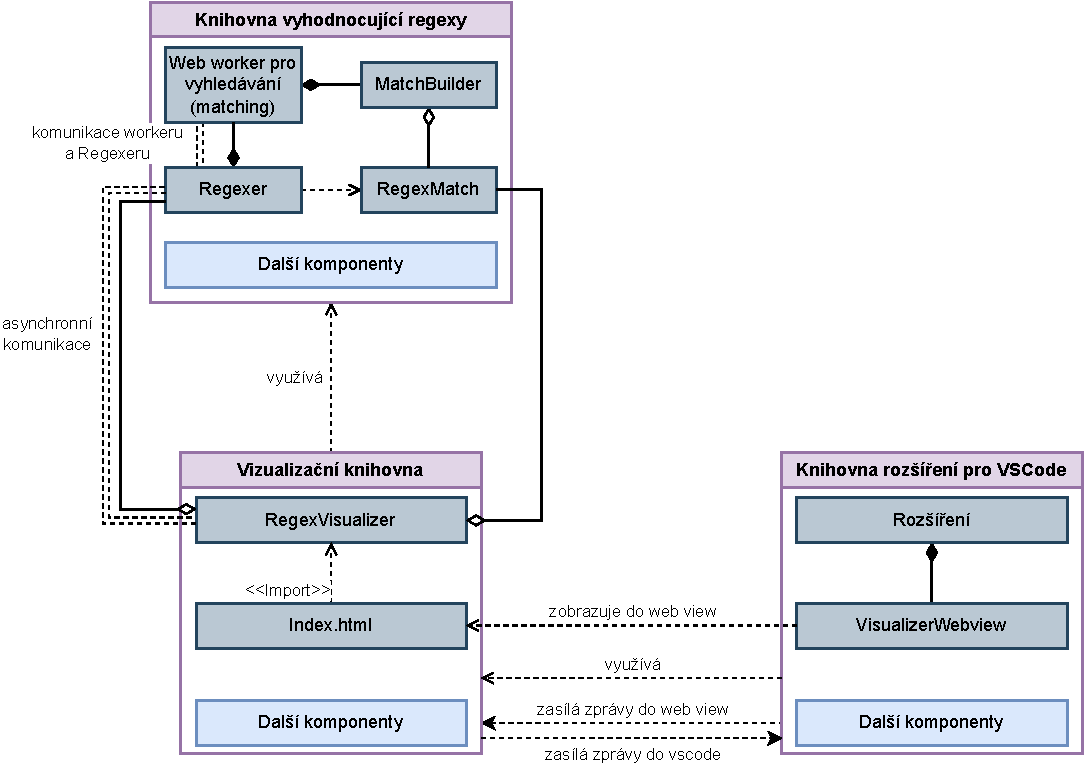
\includegraphics[width=0.8\textwidth]{Figures/BP-Arch.pdf}
	\caption{Struktura knihoven aplikace}
	\label{fig:ARCH}
\end{figure}

\newpage

\section{Použité technologie}\label{sec:USEDtech}
Tato aplikace je integrovaná do vývojového prostředí \textbf{visual studio code}, 
zkráceně \textbf{vscode}. Jádro aplikace je psáno v programovacím jazyce \textbf{TypeScript}, zkráceně \textbf{TS} verze 5.3, který je nádstavbou
pro jazyk \textbf{JavaScript}, zkráceně \textbf{JS}. TypeScript, jak z názvu vyplívá je typový JavaScript.
Každý kód napsaný v JS je správný pro TS, ale to neplatí naopak.
Psaní nějaké větší aplikace je tak vhodnější v TS, 
kvůli svím typovým kontrolám, čímž se můžeme vyhnout potencionálním chybám v běhu programu.
Také vyvýjení rozšíření pro vscode, je možné pouze v JavaScriptu nebo TypeScriptu.

Pro parsování je použita bezkontextová gramatika Peggy\cite{Peggy, Peggyjs}, pro jazyk JavaScript.
Ta umožňuje poměrně snadného zpracování textové podoby regulárních výrazů do podoby strukturované.
Tato výsledná struktura může být vpodstatě jakákoliv.

Části aplikace jsou zpravovány balíčkovým manažerem \textbf{NPM} (Node Package Manager).
Využívají tedy balíčků, které jsou dostupné pro npm. 
Aplikace je pak postavená na technologii \textbf{NodeJS}, 
jedná se o JavaScript runtime (běh programu). 
Runtime vscode rozšíření je totiž NodeJS, ale samotné web view běží na klasickém webovém runtime, které je typické pro webové prohlížeče.

Visualizační část aplikace pak využívá základní \textbf{HTML} struktury.  
HTML je základem pro webové stránky a definuje jejich strukturu pomocí značek.
Pro následné stylování, je využito technologie \textbf{LESS}, což je rozšíření standartního \textbf{CSS}.
Avšak LESS musí být transpilovaný\footnote{Typ překladu z jednoho jazyka na jazyk jiný} do CSS, jelikož webová stránka ho nezná. 
LESS umožňuje, například vnořování stylů nebo tvorbu vlastních proměnných.
Pro logickou část visualizační knihovny je také využit TypeScript.

Pro výsledný přeložený kód, je použit balící nástroj \textbf{webpack}.
Ten nám umožňuje, všechny části aplikace poměrně efektivně zabalit, do malého počtu souborů. 
Tento nástroj se pak hodí, pro menší výslednou aplikaci a hlavně pro seskupení všech závislostí.
Můžeme mít i větší kontrolu nad výsledným kódem.
Například můžeme udávat kdy se mají soubory dělit, jak se mají zpracovávat přílohy, jako jsou obrázky atd.
Pro optimalizaci a úpravu kódu, se zde využívá takzvaných \textbf{loaderů} a \textbf{pluginů}, 
které dokážou v určité části překladu zasáhnout a popřípadě změnit určitou část kódu.
Ve výsledku se jedná o velice silný nástroj, který dává programátorovi větší kontrolu nad výsledným přeloženým kódem aplikace.

Jelikož chceme mít větší jistotu správnosti aplikace, je v logické části aplikace využito technologie pro tvorbu testů. 
Tato knihovna se nazívá \textbf{Jest}, protože je tato knihovna převážně pro testování JavaScriptových kódů, 
tak je s ní využito pro TypeScriptové soubory \textbf{ts-jest}. To nám pak umožňuje psát testy určené i pro typovost TS.

Jednou z posledních knihoven, která je použita je \textbf{threads.js}. 
Jelikož existují různé runtime JavaScriptu, tak neexistuje jednotné využití vláken (threadů).
Browser má tzv. \textbf{web workery} a NodeJS má \textbf{worker thready}, sice si jsou podobné, ale mají změny které znemožňují univerzálního použití.
Proto je v této aplikaci využito knihovny threads.js, která eliminuje tyto problémy.
Navíc dokáže zpřístupnit větší bezpečnost pro programátora, který píše kód v TS. 
Tato bezpečnost je docílená tím, že knihovna umožňuje poskytnout z vlákna rozhraní, které může obsahovat i typy.
Základní funkcionalitu knihovny threads.js lze vidět, v ukázce zdrojového kódu \ref{code:threads}.

\begin{code}[!ht]
	\begin{minted}{typescript}
/* --------- Hlavní vlákno --------- */
/* Zavolání metody workera z rodiče */
await this.worker_?.match(pid, matchString, options?.batchSize ?? -1);

/* --------- Worker --------- */
const Matcher = {
	match(pid : number, matchString : string, batchSize: number = -1) : 
	ReturnMatch | ReturnBatch | ReturnAborted | null
	{
		// logika funkce
	}
}
expose(Matcher); /* Zviditelnění objektu Matcher pro rodiče */
	\end{minted}
	\caption{Příklad použití knihovny threads.js}
	\label{code:threads}
\end{code}

\newpage

Workery v JS, jsou limitovány tím, že komunikace mezi hlavním a vedlejším vláknem, probíhá formou zpráv.
Demonstraci této komunikace lze vidět ve zdrojovém kódu \ref{code:worker}.
U příjmutých zpráv nemůžeme zjistit před během programu, co nám z vlákna příjde za odpověď. 
Na to si programátoři, musí dávat pozor, aby předešli chybám, které mohou nastat při běhu programu.
Knihovna threads.js sice na pozadí volá buď worker thread nebo web worker, podle prostředí ve kterém běží, 
ale poskytuje rozhraní, které je programátorsky přijatelnější.

\begin{code}[!ht]
	\begin{minted}{typescript}
/* --------- Hlavní vlákno --------- */
/* poslání zprávy do workeru */
myWorker.postMessage({type: "match", pid, matchString, batchSize});

myWorker.onmessage = (event : MessageEvent)
{
	// event.data má typ any (neznámý), jedná se o poslanou proměnnou message 
	// kontrola dat například pomocí switche
}

/* --------- Worker --------- */
onmessage = (event : MessageEvent) => {
	// stejná situace, která je u hlavního vlákna onmessage

	/* poslání zprávy zpět do hlavního vlánka */
	parentPort.postMassage(message);
}
	\end{minted}
	\caption{Příklad použití web workeru a posílání zpráv}
	\label{code:worker}
\end{code}
% TODO: popsat peggy syntax
\endinput